%!TEX root = finalReport.tex
%!TEX encoding = UTF-8 Unicode
%==============================================================================

	Industrial robots are reshaping the present and future of most, and very soon all, industrial aspects. They are currently used in a broad spectrum of industries, some of which include car parts assembly as in BMW and Mercedes factories, industrial automation as in Yaskawa factories, metal industries that include welding and machining processes and many others. While there is a controversial part in replacing humans with robots in factories, it, nevertheless, offers more accuracy and higher production rate with more space for development. The growth of the Global Industrial Robotics Market is driven by many factors, of which the need to reduce manufacturing cost in industries is one of the main drivers. Industrial robotics aids companies in reducing the cost due to product failure and product wastage.
    
Some of the pioneering companies in the Industrial robotics market are ABB Ltd., Fanuc Corp., Yaskawa Electric Corp., Apex Automation and Robotics, Mistubishi Electric Corp. and KUKA AG. We had the opportunity to work with the latter, KUKA AG, on the implementation of our project (\emph{ZuKa: Deployment of the industrial KUKA robotic manipulator in CNC machining and visual servoing through Kinect interfacing on ROS}). Over the course of our final year, this project helped increase our knowledge, not only on the main topic, machining and visual servoing, but also on the KUKA platform itself, which is considered an advanced platform widely used in today’s industries. 

The project is inspired by the aforementioned development in the industrial sector. The scope of the project can be summarized in the following three points; firstly, the commissioning and operation of the KUKA KR6 R900 sixx robotic manipulator, which included the installation of the related software and creating a network that facilitates communications with the robot. In addition to software commissioning, hands-on experience with the KUKA robot language (KRL) platform was achieved through learning the basic and advanced forms of KRL, which later helped in the development of software tools that facilitates the main objective of the project; the milling process. 

Secondly, the design and manufacturing of a base to support the robot during heavy duty operation, this included performing mathematical calculations based on the robot’s weight and forces to obtain the optimal dimensions and weight for the base, besides performing CAD studies on the manipulator’s body to support the results of the mathematical analysis. 

Finally, the development of various software tools to achieve the purposes of remotely controlling the robot and milling. These tools include an Inkscape extension for converting 2D G-code to KRL, directly using sketches from Inkscape, an independent toolkit for converting 3 axis G-code to KRL. In addition to Python tools; one Python class for reading and writing system variables, and a Python library for controlling the arm motions from pc. The development also included editing openni\_tracker for publishing uncalibrated person's depth and creating ROS nodes for safety operation distance and visual servoing (hand guiding) for the robot.

Initially, the project scope was limited to the milling process in addition to minor ideas in the smart development of the workspace, however, over the course of the semester we encountered many problems that required extended research in all the previously mentioned aspects, which eventually led to broadening the scope of the project to include these development tools, both relevant and irrelevant to milling. 
\begin{figure}[h]
    \centering
    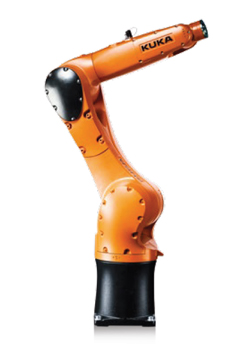
\includegraphics[width=0.7\linewidth]{figures/kuka}
    \caption[test Fig]{This is a test figure. You can use it as a template for your figures}
    \label{fig:kuka}
\end{figure}

\section{Project Contributions}
The results of the project studies and implementation include, but not limited to; 
\begin{itemize}
\item	The manufacturing of the robot’s base, with mathematically calculated data endorsed by CAD studies, contributing in a stable, secure and robust base that can support the weight of the robot and tolerate the forces resulting from the robot’s motion without major failure or errors.

\item	The attachment and operation of a pneumatic gripper, leading to the development and implementation of software tools for drawing and palletizing.

\item	The development of different software tools to obtain the appropriate KRL codes used in the milling process.

\item	The development of a safety system in the robot’s workspace, similar to KUKA AG’s own Collision detection, which stops thee robot from moving when it hits a solid surface. However, being more efficient and safe, in terms that it does not require actual contact or collision but significantly reduced the operation speed of the robot when someone enters a defined perimeter of the robot’s workspace. This is achieved using a Microsoft Kinect device for obtaining visual input of the workspace.
\end{itemize}

The results of the work exceeded both the preset expectations and goals for the project, resulting in a wide variety of applications and an extension in our own knowledge base, which is the most important achievement. 


%==============================================================================

%just some text for text
%\section{overview}
%some data
%\subsection{Flower Power}
%
%\begin{figure}[h]
%    \centering
%    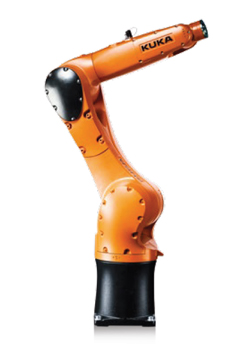
\includegraphics[width=0.7\linewidth]{figures/kuka}
%    \caption[test Fig]{This is a test figure. You can use it as a template for your figures}
%    \label{fig:kuka}
%\end{figure}
